\subsubsection{Stepper-Motor}
    Der Motor der die Ausrichtung des Werfers vornimmt muss sehr genau und reproduzierbar die Ausrichtung vornehmen. Aus diesem Grund wird ein Stepper-Motor eingesetzt. Die Ansteuerung dieses Motors wird in der ET-Gruppe erarbeitet und hier verwendet. Die entsprechende Dokumentation ist im Anhang \ref{Stepper_Dokumentation} angehängt.
    %
\subsubsection{DC-Motor}
    Der Antrieb des Förderbands muss nur in einer Richtung funktionierten. Deshalb ist die Ansteuerung besonders einfach. Die Steuerung des DC-Motors erfolgt mittels eines PWM-Signals, das über einen entsprechenden Transistor direkt angesteuert wird. Abbildung \ref{fig:Schema_DC-Motor} zeigt, wie die Ansteuerung des DC-Motors umgesetzt wird.
    \begin{figure}[h!] %{0.45\textwidth}
    	\centering
    	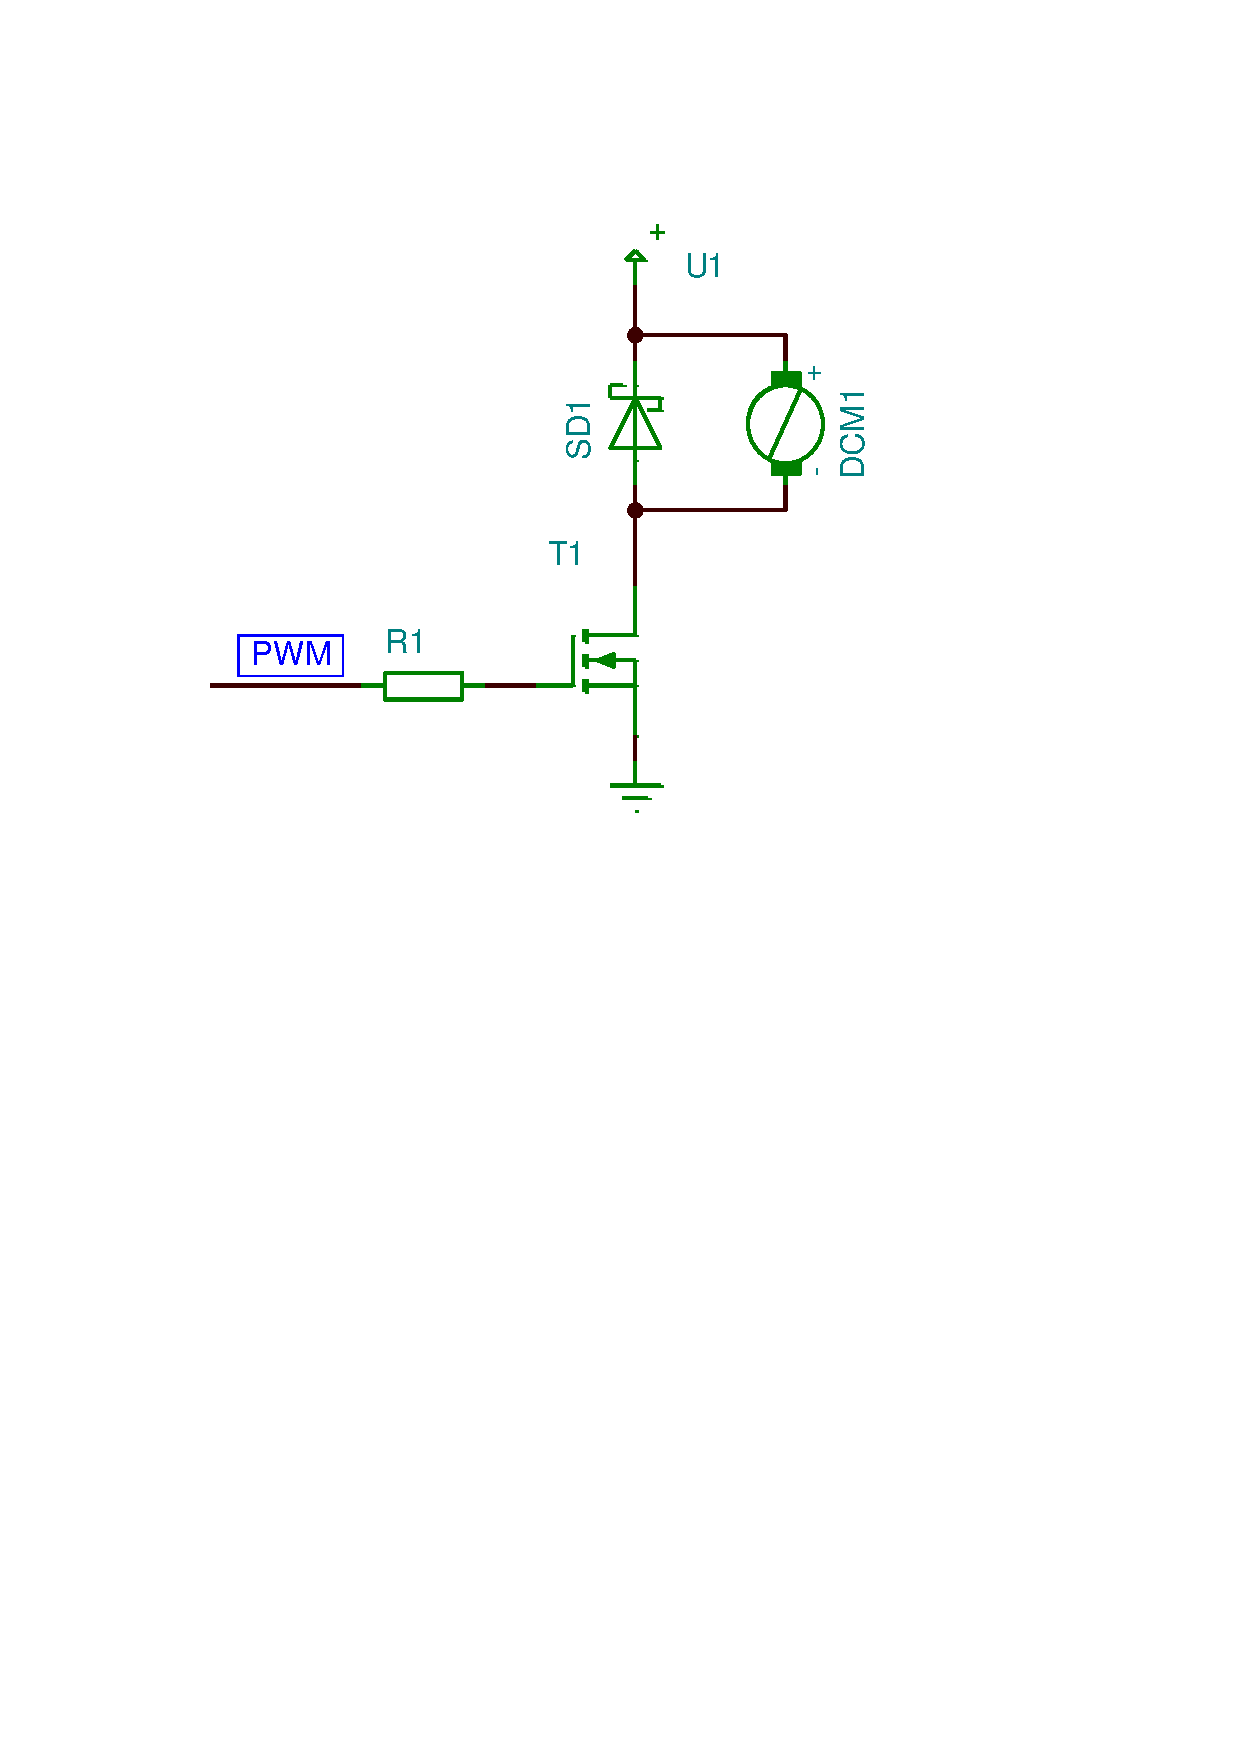
\includegraphics[width=0.5\textwidth,clip,trim=37mm 159mm 62mm 37mm]
    	{Enddokumentation/Loesungskonzept/Bilder/SchemaDcMotor.pdf}
    	\caption{Schema der DC-Motoransteuerung}
    	\label{fig:Schema_DC-Motor}
    \end{figure}